\chapter{Detector Design and Construction}\label{chapter:setup}

\section{Introduction \& Motivation}

\section{Detector Concept \& Scintillator Selection}\label{section:detector:concept}
Two different scintillation-based detector-concepts were developed to measure the depth dose distribution of protons in real-time.
Both detectors consist of 32 scintillator-layers read-out via \glspl{SiPM} and two linked-together 16-channel CAEN digitizer.

The first detector concept is \ce{PbWO4}-based, as the first prototype,  [citemaster], but improves on the layer geometry by using sheets instead of bars whilst also reducing layer thickness.
For this two crystal sizes were chosen with $30\times30\times3~\text{mm}^3$ and $30\times30\times2~\text{mm}^3$, which were provided and cut by Crytur, allowing full coverage of the \SI{220}{\mega\electronvolt} proton range of $\approx \SI{66}{\mm}$.
The lateral sheet sizes with \SI{30}{\mm} were the largest providable, because the sheets were cut from a single ingot and the thicknesses are the smallest resonable due to \ce{PbWO4} being very fragile.
The \SI{3}{\mm} thick sheets are used in the front or shallow beam depths to provide more stopping power and the thinner \SI{2}{\mm} sheets are used in the Bragg-Peak region to give an optimal spatial resolution.

The second detector concept using plastic scintillators was developed to further increase the spatial resolution in the Bragg-Peak region at the cost of dynamic range in the shallow depths. 
Plastic scintillators were chosen because they have a much lower density and thereby stopping power than \ce{PbWO4} and a high light yield also giving a better energy resolution.
However, to achieve a high spatial resolution whilst using only 32 channels, individual channls need a low radiological thickness resulting in not fully covering the proton range.
To still stop the proton beam, a passive absober with a known stopping power i.e. radiological thickness is incorperated between the first and second scintillator layers.
This allows the first to work as a trigger channel which is used for the normalization in the analysis.

\section{Detector Simulation}
Geant4 simulations of both detector designs were implemented to give insights into their respective performances and to strike a good balance between active and passive volume for the plastic based detector.

\subsection{Detector Implementation}
The \ce{PbWO4} based detector was implemented as 32 \ce{PbWO4} sheets 
The scintillators are wrapped in \SI{0.5}{\mm} PTFE-foil and \SI{20}{\um} aluminum foil.
Here PTFE is modeled after its molecular formula of the repeating unit \ce{C2F4} with a density of $\rho_{\text{PFTE}}=\SI{2.2}{\gram\per\cm\cubed}$ and a mean exictiation energy of $I_{\text{PTFE}} = \SI{99.1}{\electronvolt}$  [citationneeded] and the aluminum foil (\SI{99.9}{\percent}) is approximated by aluminum. 

The plastic based detector was implemented using an active and passive material.
The active material was modeled after a PVT-based scintillator, similar to general purpose plastic scintillators like EJ-200 or BC-408.
Here, the material is composed out of hydrogen and carbon with the mass fractions of \SI{8.5}{\percent} and \SI{91.5}{\percent}, respectively [citeEJ].
The passive material is PMMA and modeled after its molecular formula of the repeating unit \ce{C5H8O2} with a density of $\rho_{\text{PMMA}}=\SI{1.9}{\gram\per\cm\cubed}$ and a mean exictiation energy of $I_{\text{PMMA}} = \SI{74}{\electronvolt}$ [citationneeded]. 
Here, the scintillators are again wrapped in PTFE and aluminum foil.

From Equation~\ref{} follows that a \SI{220}{\mega\electronvolt} proton beam has a range of \SI{30.45}{\cm} in water.
Considering that plastic scintillators have a very similar stopping power and that the Bragg-Peak region is about 1/3 of the depth-dose distribution this leads to a scintillator thickness of $\approx\SI{4}{\mm}$.
For the 32 available channels this gives a coverage of $\approx \SI{12.8}{\centi\meter}$ of the \SI{30.45}{\centi\meter} proton range, resulting in a $\approx\SI{20}{\cm}$ passive absorber.
To chose the right thickness of the PMMA absorber, its water equivalent radiological thickness after the first scintillator layer has to be calculated.
This is done using the total energy deposition inside the absorber by integrating Equation~\ref{}(range energy), as shown in Equation~\ref{eq:detector:absorber:thickness}.

\begin{align}
    \label{eq:detector:absorber:thickness}
    \Delta E_{\ce{H2O}} &= \Delta E_{mat} \\
    \int_{z_n}^{z_{n+1}} S_{\ce{H2O}}\text{d}z &= \int_{x_n}^{x_{n+1}} S_\text{mat}\text{d}x \\
    E(z_{n+1})_{\ce{H2O}}-E(z_n)_{\ce{H2O}}&= E(x_{n+1})_{\text{mat}}-E(x_n)_{\text{mat}}\\
    E(z_n)_{\ce{H2O}} = E(x_n)_{\text{mat}} \rightarrow E(z_{n+1})_{\ce{H2O}} &= E(x_{n+1})_{\text{mat}} \\
    x_{n+1} = x_n + \Delta x \rightarrow \left(\frac{z_{n+1}}{\alpha_{\ce{H2O}}}\right)^{\frac{1}{p_{\ce{H2O}}}} &= \left(\frac{x_{n}+\Delta x}{\alpha_{\text{mat}}}\right)^{\frac{1}{p_{\text{mat}}}} \\
    x_{n} = \alpha_{\text{mat}} \left(\frac{z_n}{\alpha_{\ce{H2O}}}\right)^{\frac{p_{\text{mat}}}{p_{\ce{H2O}}}} \rightarrow z_{n+1} &= \alpha_{\ce{H2O}} \left(\left(\frac{z_n}{\alpha_{\ce{H2O}}}\right)^{\frac{p_{\text{mat}}}{p_{\ce{H2O}}}} + \frac{\Delta x}{\alpha_{\text{mat}}}\right)^{\frac{p_{\ce{H2O}}}{p_{\text{mat}}}}
\end{align}

The water equivalent thickness 

\section{Readout}\label{section:readout}
The scintillators of both designs are read out via SiPMs.
Light yield measurements were conducted, to decide which SiPM types are suitable.
With these the amount of incident photons can be estimated and compared with the number of pixel.
From this, a balance can be struck between high resolution and a large enough dynamic range.
 
\subsection{Light Yield Measurement}
The measurements were conducted using the process described in Section~\ref{section:lightyield} and the setup shown in Figure~\ref{fig:lightyield:setup}.
The PMT used is an R2059 from Hamamatsu (serial number BA3200) with a quantum efficiency of \SI{23.16}{\percent}~\cite{datasheet:hamamatsu_R2059} (cf. Appendix~\ref{appendix:spectral}) at the luminescence peak of \SI{420}{\nano\meter} of \ce{PbWO4}~\cite{cms:tdr} and EJ212.

\subsubsection{Light Yield: \ce{PbWO4}}
The \ce{PbWO4} measurement were done in a flat and vertical position as shown in Figure~\ref{fig:lightyield:pwo:setup}, where all non PMT-facing scintillator sides were enveloped in highly reflective PTFE foil in order to not lose any photons.
Two additional measurements were performed, where one \SI{3}{\milli\meter}- and \SI{2}{\milli\meter} crystal were fully wrapped with an SiPM sized window cutout in the center of one side  as shown in Figure~\ref{fig:detector:crystal:pwo:wrap}.
The \ce{PbWO4} crystals were mounted onto the PMT's optical window next to a \ce{^{22}Na} $\gamma$-source inside a climate chamber.
The optical coupling was done using glycerol ($n=1.4722$), as shown in Figure~\ref{fig:pwo:lightyield:open}.
Glycerin was used as a substitute for the commonly used Baysilone\textsuperscript{{\textregistered}} Fluid~M optical grease ($n\approx 1.404,~\eta=\SI{300000}{\milli\meter^2\per\second}$~\cite{bayer:baysilone}), due to its less-adhesive characteristic.
The Baysilone\textsuperscript{{\textregistered}} Fluid~M with its high adhesion might have lead to damaging the fragile crystals during removal.
The refractive index of \ce{PbWO4} and the \ce{SiO2} glass window of the \gls{PMT} are $n_{\ce{PbWO4}}\approx2.3$~\cite{cms:tdr} and $n_{\ce{SiO2}}\approx1.459$~\cite{Malitson:65}, respectively.
Additionally to the climate chamber's light-tightness, the setup is enclosed in PTFE foil, ensuring perfect light tightness.

\begin{figure}[h]
    \centering        
    \subfloat[Flat position.\label{fig:lightyield:pwo:setup:f}]
        {\includegraphics[width = 0.45\textwidth]{fig/lightyield/pwo/ly_pwo_flat.jpg}}
    \hspace{0.02\textwidth}
    \subfloat[Vertical position.\label{fig:lightyield:pwo:setup:v}]
        {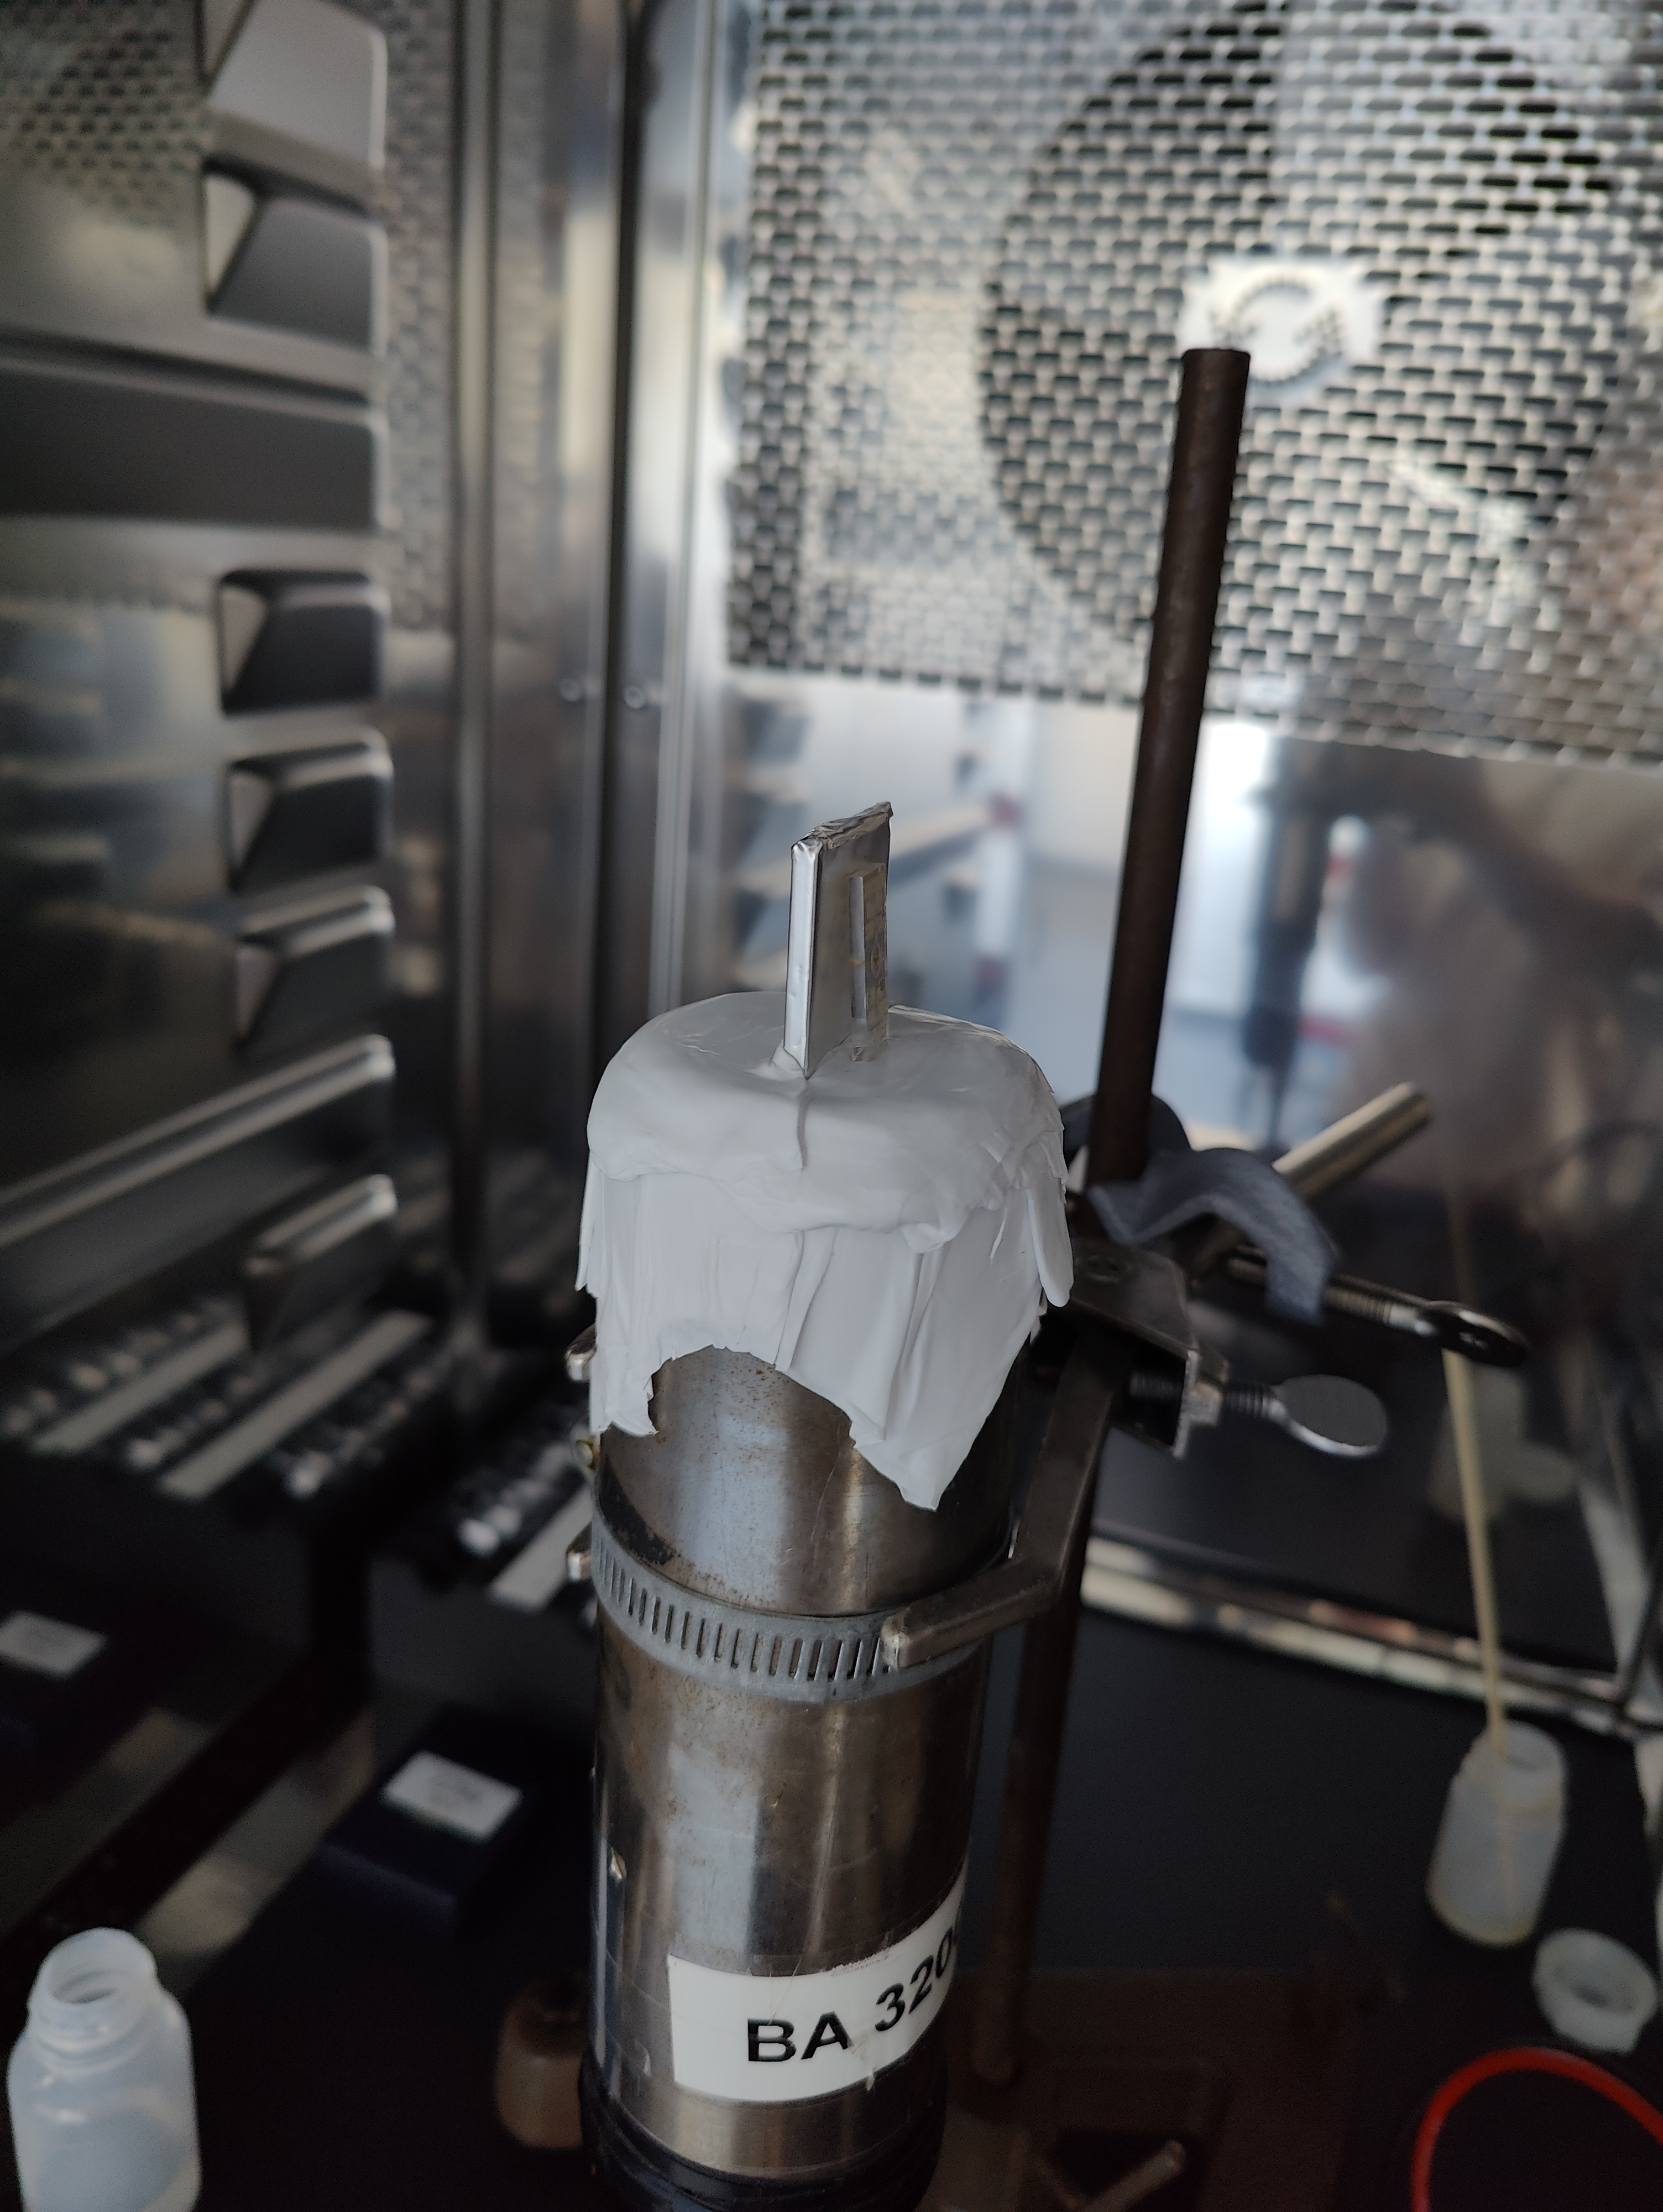
\includegraphics[width = 0.45\textwidth]{fig/lightyield/pwo/ly_pwo_vertical.jpg}}\\ 
    \caption{Measurement positions of the \ce{PbWO4} scintillators on the \gls{PMT} for the light yield measurements using a \ce{^{22}Na} source.}\label{fig:lightyield:pwo:setup}
\end{figure}


The measurements were conducted at \SI{20}{\celsius} for \SI{5}{\minute} after an acclimation time of \SI{5}{\minute} each.
The acclimation time was chosen small because the crystals were keept inside the climate chamber for \SI{24}{\hour} before the measurements were startet, thereby only the short time frame inbetween measuements, where the chamber was opened, had to be accounted for.
An exemplary light yield measurement of crystal number~0 in the flat position is shown in Figure~\ref{fig:lightyield:pwo:measurement:0}.
The measured light yield values of all crystals and their averages for the different setups are shown in Figure~\ref{fig:lightyield:pwo:measurement:all}.
The \SI{3}{\milli\meter} thick crystals average approximately \SI{164.73}{ph\per\mega\electronvolt} and \SI{129.44}{ph\per\mega\electronvolt} in the flat and vertical positions, respectively.
The \SI{2}{\milli\meter} thick crystals average approximately \SI{131.00}{ph\per\mega\electronvolt} and \SI{94.32}{ph\per\mega\electronvolt} in the flat and vertical positions, respectively.
With the SiPM-sized window cutout the light yield of a \SI{3}{\milli\meter} and \SI{2}{\milli\meter} crystal was \SI{75.25\pm 33.09}{ph\per\mega\electronvolt} and \SI{59.7\pm 19.22}{ph\per\mega\electronvolt}, respectively.

\begin{figure}[h]
    \centering
    \includegraphics[width=0.5\linewidth]{fig/lightyield/pwo/bps_na_flat.pdf}
    \caption{Example light yield measurement of the \SI{3}{\milli\meter} thick \ce{PbWO4}-crystal number 0 in flat position on the \gls{PMT} using a \ce{^{22}Na} source.}\label{fig:lightyield:pwo:measurement:0}
\end{figure}

\begin{figure}[h]
    \centering
    \includegraphics[width=1\linewidth]{fig/lightyield/pwo/bps_na22_all.pdf}
    \caption{Light yield measurements of \ce{PbWO4}-crystals in flat and vertical positions including two window cut-out measuremetns using a \ce{^{22}Na} source.}\label{fig:lightyield:pwo:measurement:all}
\end{figure}

\subsubsection{Light Yield: EJ-200}
The light yield of a $50 \times 50 \times 10~ \si{\milli\meter\cubed}$ EJ-200 sample was measured to estimate the amount of incident photons on an SiPM optically coupled to an EJ-212 scintillator, which has similar properties to EJ-200, to decide which SiPM type is needed for the readout.

The measurements were done in a flat and vertical position, with two source positions for the vertical setup, as shown in Figure~\ref{fig:lightyield:ej200:setup}.
In the vertical position two wrappings for the scintillator were used.
First the whole PMT facing side was left open and secondly only an \gls{SiPM}-sized window cutout was left open.
The scintillator was mounted onto the PMT's optical window inside a climate chamber and optically coupled using Baysilone\textsuperscript{{\textregistered}} Fluid~M optical grease~\cite{bayer:baysilone}.
The setups were fully enclosed in PTFE foil to ensure light-tightness.
The source positions were on the side and on top of the scintillator.
A \ce{^{241}Am} source was chosen due to the high light yield of EJ200 as \ce{^{241}Am} has a prominent low-energy gamma line at \SI{59.6}{\electronvolt}.

\begin{figure}[h]
    \centering        
    \subfloat[Flat position.\label{fig:lightyield:ej200:setup:f}]
        {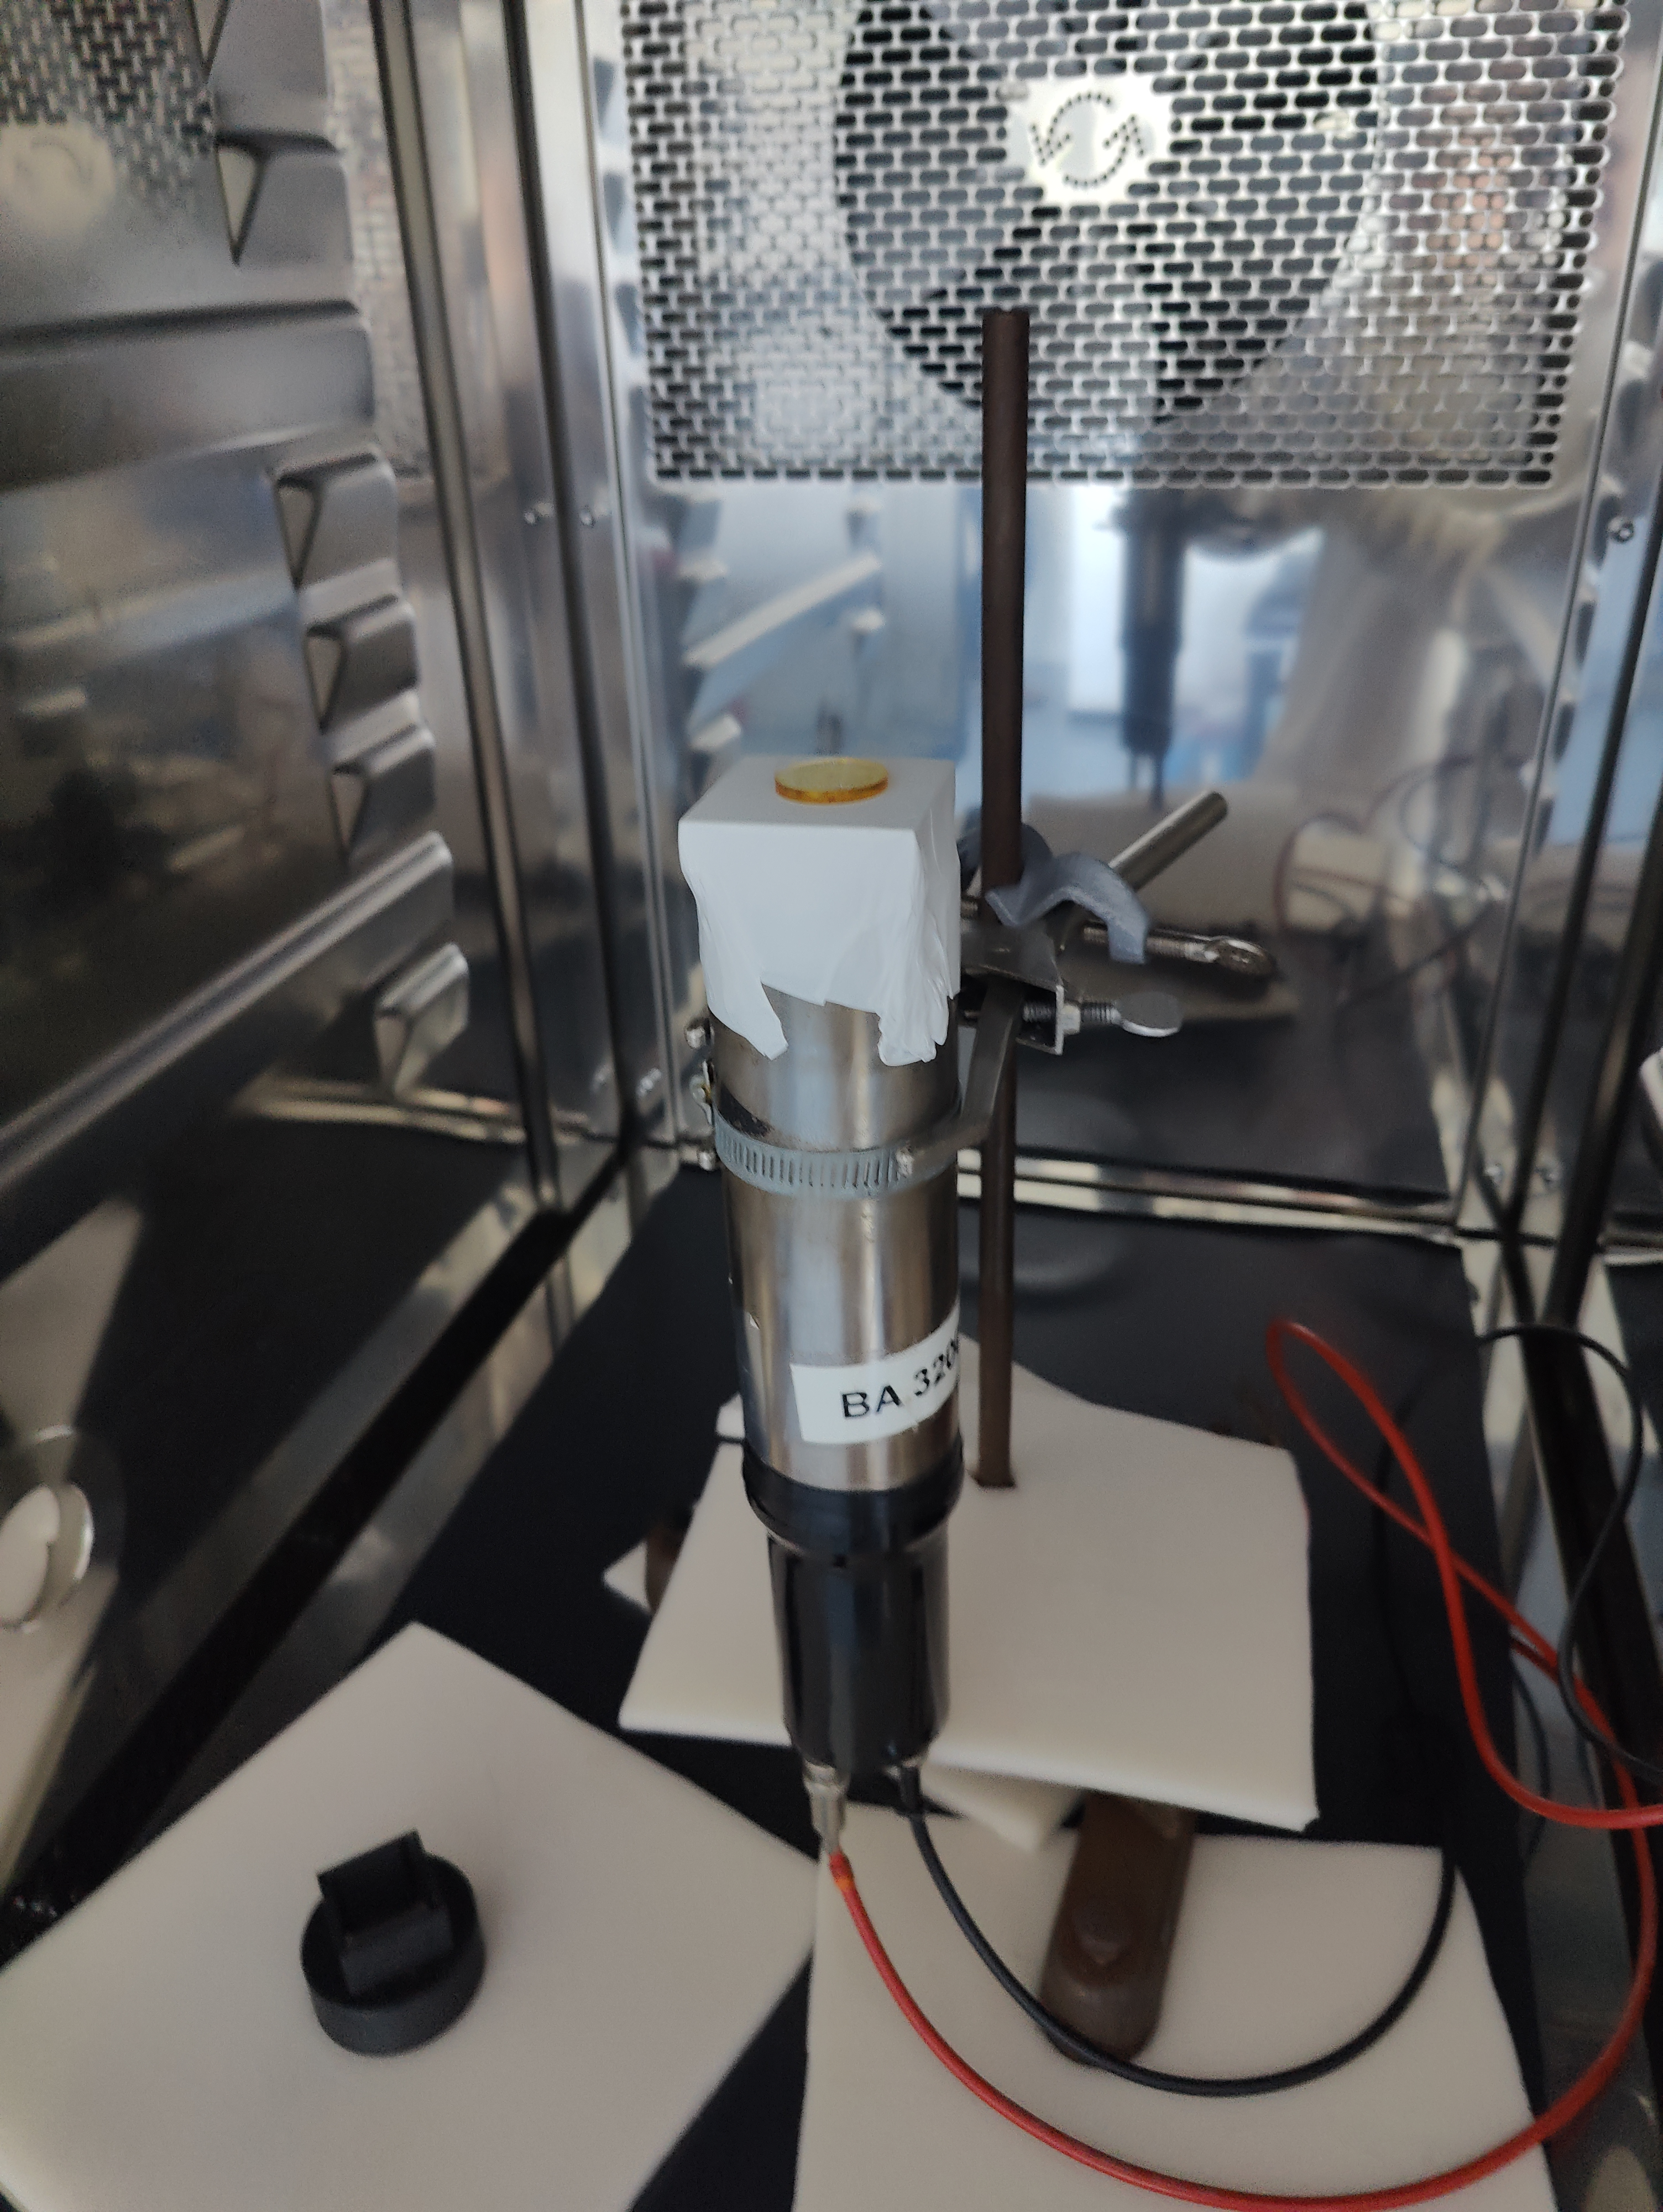
\includegraphics[width = 0.45\textwidth]{fig/lightyield/ej200/ly_ej200_flat.jpg}}
    \hspace{0.02\textwidth}
    \subfloat[Vertical position.\label{fig:lightyield:ej200:setup:v}]
        {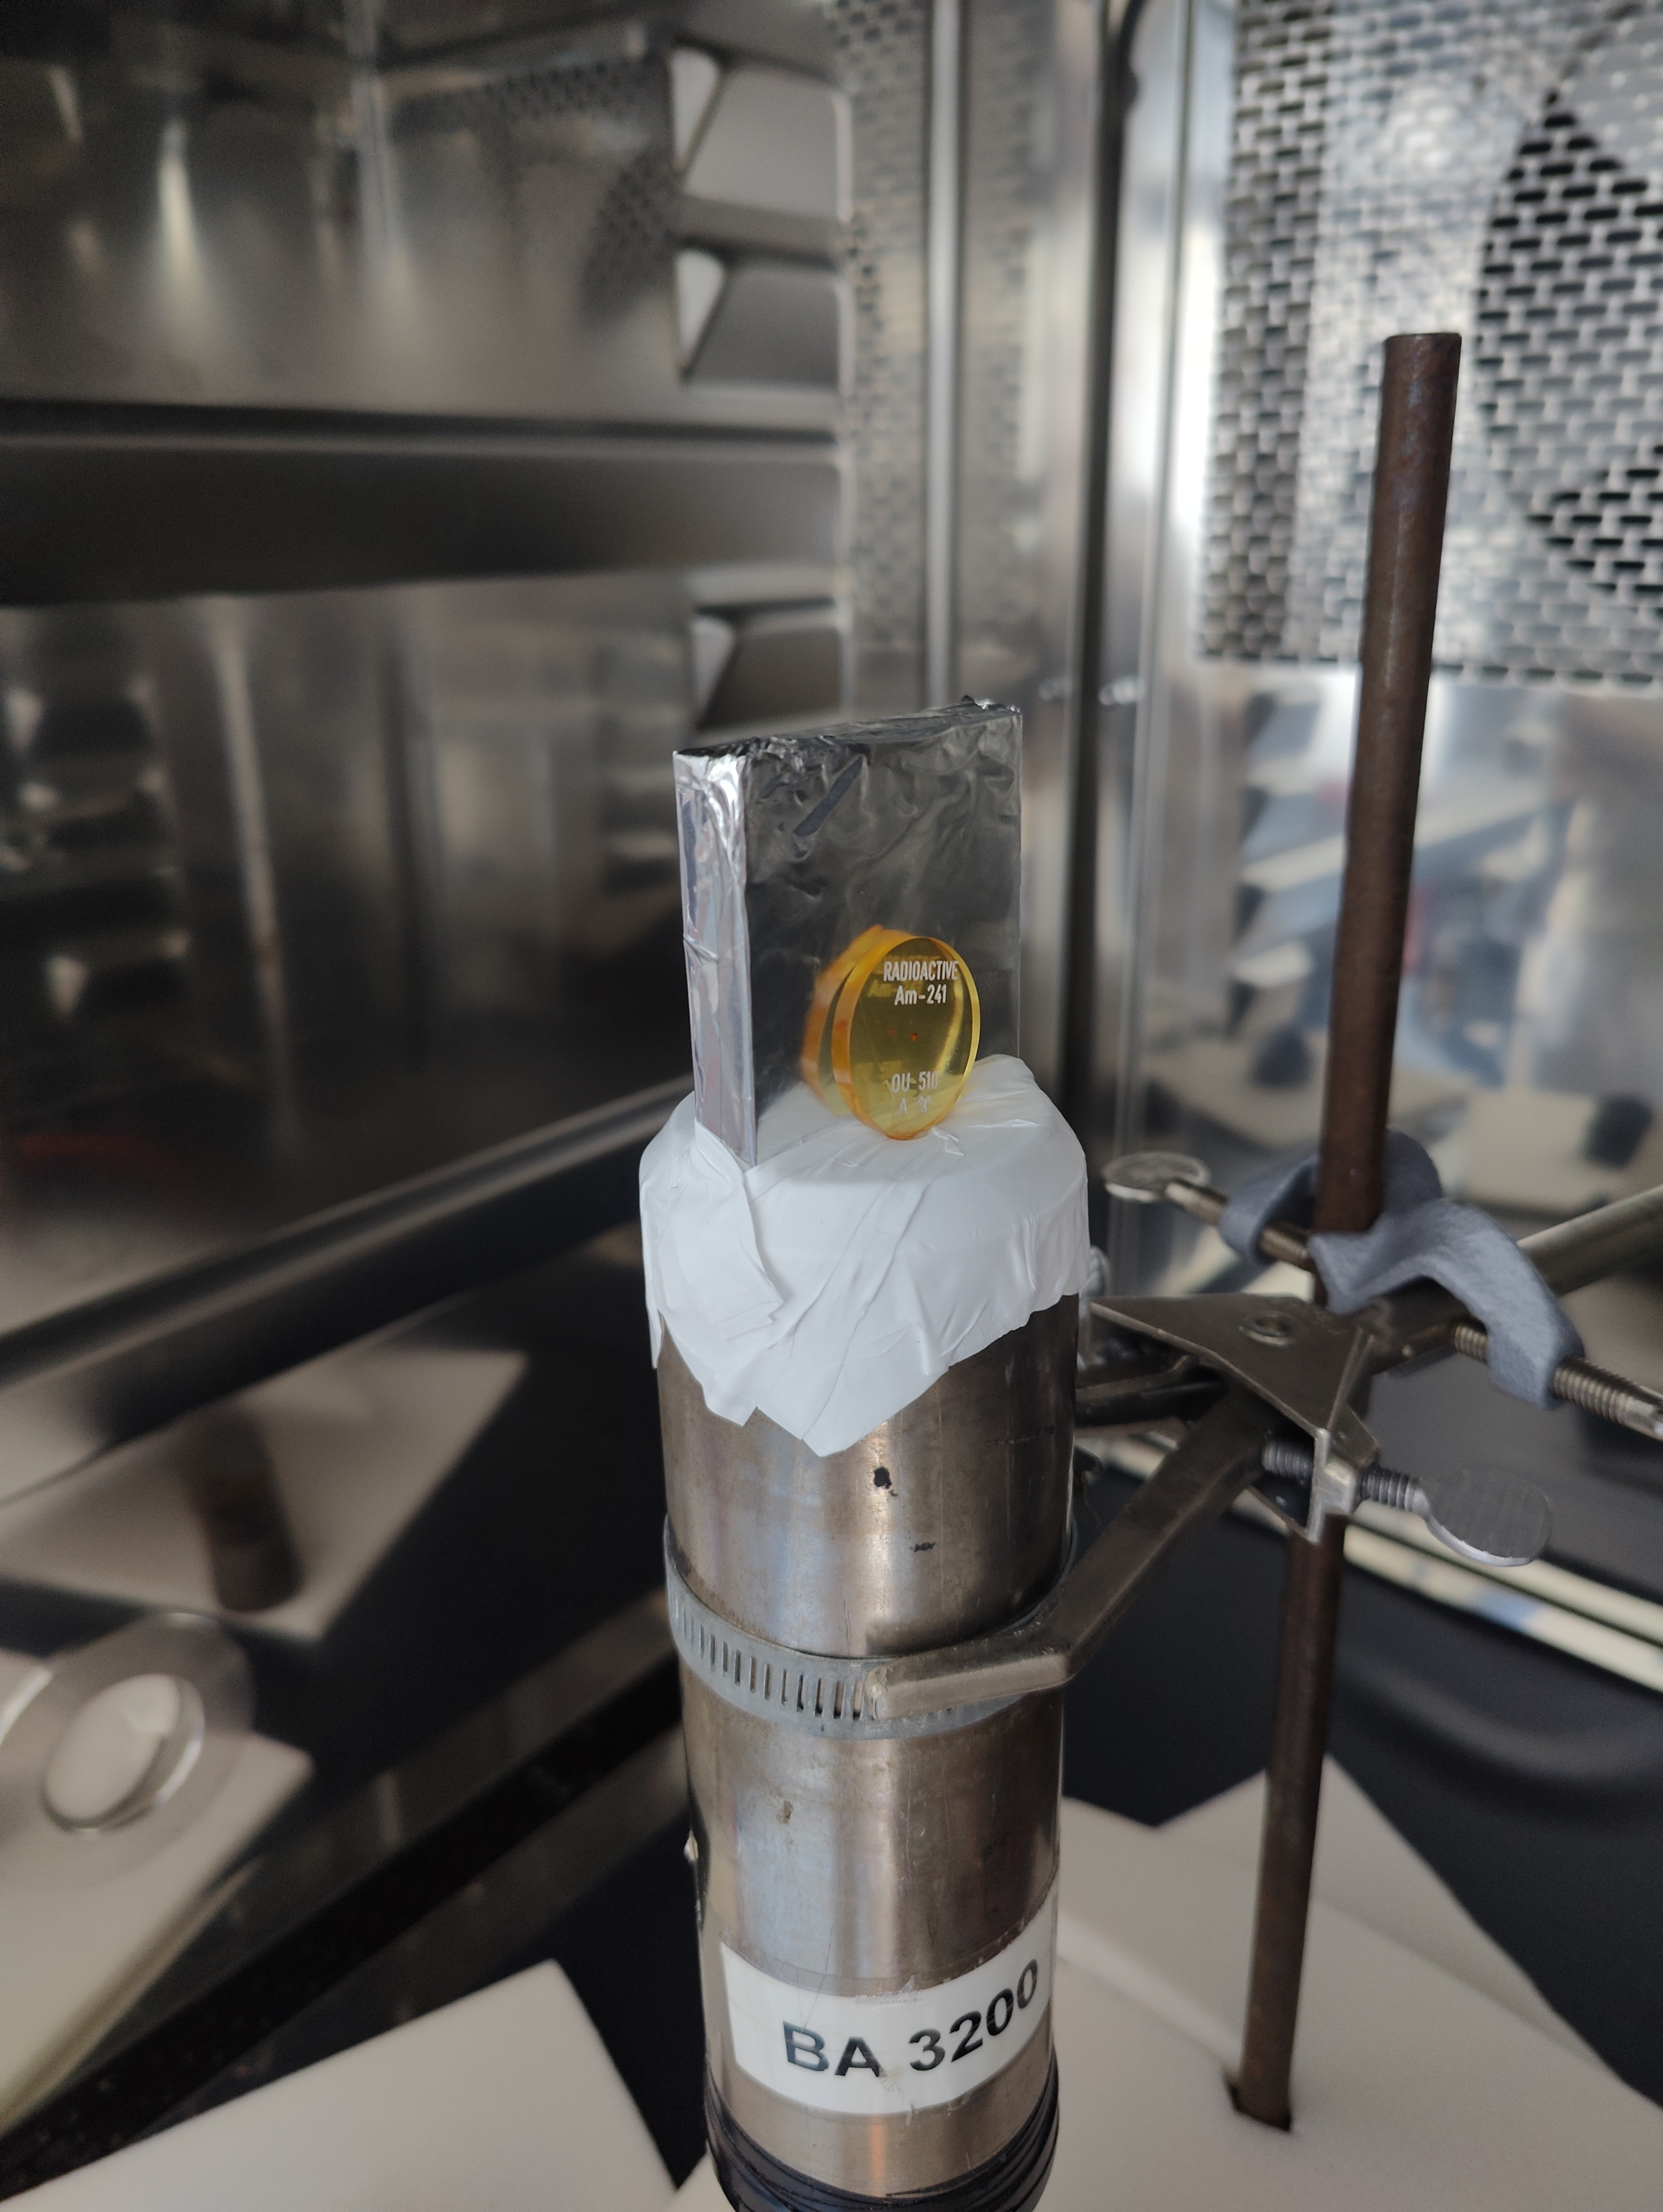
\includegraphics[width = 0.45\textwidth]{fig/lightyield/ej200/ly_ej200_vertical.jpg}}\\ 
    \caption{Measurement positions of the EJ-200 scintillator on the \gls{PMT} for the light yield measurements using a \ce{^{241}Am} source.}\label{fig:lightyield:ej200:setup}
\end{figure}

The measurements were conducted at \SI{20}{\celsius} for \SI{20}{\minute} after an acclimation time of \SI{24}{\hour}.
The measurements and Gaussian fits of the \SI{59.6}{\electronvolt} peak are shown in Figure~\ref{fig:lightyield:ej200:measurement}.

\begin{figure}[hp]
    \centering
    % Top row
    \makebox[\textwidth][c]{%
    \begin{subfigure}[t]{0.48\textwidth}
        \includegraphics[width=\textwidth]{fig/lightyield/ej200/bps_ej200_flat.pdf}
        \caption{Flat scintillator position.}\label{fig:lightyield:ej200:measurement:0}
    \end{subfigure}
    }
    \vspace{0.5cm}
    % Bottom row (2 images, centered)
    \begin{subfigure}[t]{0.48\textwidth}
        \includegraphics[width=\textwidth]{fig/lightyield/ej200/bps_ej200.pdf}
        \caption{Vertical position with open side and source on top.}\label{fig:lightyield:ej200:measurement:1}
    \end{subfigure}
    \hfill
    \begin{subfigure}[t]{0.48\textwidth}
        \includegraphics[width=\textwidth]{fig/lightyield/ej200/bps_ej200_side.pdf}
        \caption{Vertical position with open side and source on the side.}\label{fig:lightyield:ej200:measurement:2}
    \end{subfigure}

    \vspace{0.5cm}

     % Bottom row (2 images, centered)

     \begin{subfigure}[b]{0.48\textwidth}
        \includegraphics[width=\linewidth]{fig/lightyield/ej200/bps_ej200_window.pdf}
        \caption{Vertical position with \gls{SiPM}-sized window cutout and source on top.}\label{fig:lightyield:ej200:measurement:3}
    \end{subfigure}
    \hfill
    \begin{subfigure}[b]{0.48\textwidth}
        \includegraphics[width=\linewidth]{fig/lightyield/ej200/bps_ej200_window_side.pdf}
        \caption{Vertical position with \gls{SiPM}-sized window cutout and source on the side.}\label{fig:lightyield:ej200:measurement:4}
    \end{subfigure}

    \caption{Light yield measurements of the $50 \times 50 \times 10 \si{\milli\meter\cubed}$ EJ-200 scintillator sample. Shown are the measurements of the scintillator in a flat position with a completly open side (\ref{fig:lightyield:ej200:measurement:0}), in a vertical position with open side and the source on top (\ref{fig:lightyield:ej200:measurement:1}) and on the side (\ref{fig:lightyield:ej200:measurement:2}), and in a vertical position with an \gls{SiPM}-sized window cutout with the source on top~(\ref{fig:lightyield:ej200:measurement:3}) and on the side (\ref{fig:lightyield:ej200:measurement:4}).}\label{fig:lightyield:ej200:measurement}
\end{figure}

The light yield results are shown in Table~\ref{tab:lightyield:ej200}.
The light yield for the flat position with is in good aggreement with the value provided by the manufacturer of \SI{10000}{ph\per\mega\electronvolt}, taking into account aging-related degradation of the PMT (from 2012), which reduce the quantum efficiency.
For both vertical positions, the light yield is only slightly affected by the source position.
This is due to the high attenuation length of optical photons in the scintillator of \SI{380}{\centi\meter}.
When photons are collected from one side, approximately \SI{30}{\percent} of the total light is lost and when using an \gls{SiPM}-sized window cut-out the light yield is reduced by \SI{70}{\percent}.

\begin{table}[h]
    \centering
    \begin{tabular}{l|c|c|c}
        Measurement & Peak position / ADC & Light yield / $\frac{\text{p.e.}}{\si{\mega\electronvolt}}$ & Light yield / $\frac{\text{ph}}{\si{\mega\electronvolt}}$ \\
        \hline 
        Flat & $3065.69 \pm 450.48$  & $1996.24 \pm 301.74$  & $8619.36 \pm 1302.84$ \\
        Vertical, Top & $2110.67 \pm 330.26$  & $1356.56 \pm 221.21$  & $5857.33 \pm 955.15$ \\
        Vertical, Side & $2196.13 \pm 362.80$  & $1413.80 \pm 243.01$  & $6104.49 \pm 1049.26$ \\
        Vertical, Window, Top & $948.9 \pm 210.69$  & $578.39 \pm 141.12$  & $2497.35 \pm 609.34$ \\
        Vertical, Window, Side & $975.01 \pm 241.14$  & $595.87 \pm 161.52$  & $2572.86 \pm 697.41$ \\
    \end{tabular}
    \caption{Light yield measurement results of the $50 \times 50 \times 10 \si{\milli\meter\cubed}$ EJ-200 scintillator sample.}\label{tab:lightyield:ej200}
\end{table}

\section{Photon Readout and SiPM Selection}\label{section:sipm:selection}
An optimal \gls{SiPM}-type for measuring the proton depth-dose distribution for the given scintillators needs to balance a high resolution with a high dynamic range to accurately measure the low energies in the shallow depths and the high energies in the Bragg-Peak region.
To ensure a linear \gls{SiPM} signal, the number of impinging photons needs to be less or equal to approximately \SI{10}{\percent} of the number of pixels divided by the \gls{PDE}. 


\subsection{SiPM for \ce{PbWO4}}
The light yield measurements of the teflon-wrapped \ce{PbWO4} crystals with an \gls{SiPM}-sized window cutout resulted in \SI{75.25\pm 33.09}{ph\per\mega\electronvolt} and \SI{59.7\pm 19.22}{ph\per\mega\electronvolt} for the \SI{3}{\milli\meter} and \SI{2}{\milli\meter} thick crystal, respectively.
The \gls{SiPM}-type chosen, was the already available Broadcom AFBR-S4N44P014M, with an active area of $3.72 \times 3.62~\si{\milli\meter\squared}$, a micro cell pitch of \SI{40}{\micro\meter}, $8334$ microcells and a maximum \gls{PDE} of \SI{63}{\percent} at \SI{420}{\nano\meter} coinciding with the luminescence maximum of \ce{PbWO4}.
The upper limit of the expected number of triggered pixels can be calculated using the highest simulated energy loss in the Bragg-Peak region, which is approximately \SI{40}{\mega\electronvolt}, as shown in Figure~\ref{}.
Accounting for the covered active area of the \gls{SiPM} by the \SI{2}{\milli\meter} thick crystal gives:

\begin{align}
    \frac{N(E)}{N(A)} &= E  \cdot \frac{L \cdot PDE}{N_0 \frac{A_{cov}}{A_{\gls{SiPM}}}}\\
    \frac{N(E_{max}=\SI{40}{\mega\electronvolt})}{N(A)} &=  \SI{40}{\mega\electronvolt} \cdot \frac{\SI{59.7}{ph\per\mega\electronvolt} \cdot 0.63 \frac{\text{1}}{\text{ph}}}{N_0 \cdot \frac{2\cdot3.72~\si{\milli\meter\squared}}{3.62\cdot3.72~\si{\milli\meter\squared}}} \\
    &= 0.327
\end{align}

\subsection{SiPM for EJ-212}
Since EJ-200 and EJ-212 are very similar the \gls{SiPM}-type for the EJ-212 scintillators was chosen based on the measurements of EJ-200.
The measured light yield for the teflon-wrapped EJ-200 scintillator with an \gls{SiPM}-sized cut-out with a center positioned source is \SI{2572.86}, as shown in Table~\ref{tab:lightyield:ej200}.
Due to the high light yield an \gls{SiPM}, the Hamamatsu S14160-3010PS was chosen.
This \gls{SiPM} has an active area of $3\times 3 \si{\mm\squared}$, a micro cell pitch of \SI{10}{\micro\meter}, $89984$ microcells and a maximum \gls{PDE} of \SI{18}{\percent} at \SI{460}{\nano\meter}, which is close to the luminescence maximum of \ce{EJ212} at \SI{423}{\nano\meter}.
The upper limit of the expected number of triggered pixels is again calculated using the highest simulated energy loss in the Bragg-Peak region, which is approximately \SI{20}{\mega\electronvolt}, as shown in Figure~\ref{}.
Accounting for the fully covered active area of the \gls{SiPM} this gives:

\begin{align}
    \frac{N(E)}{N_0} &= E  \cdot \frac{L \cdot PDE}{N_0}\\
    \frac{N(E_{max}=\SI{20}{\mega\electronvolt})}{N(A)} 
    &=  \SI{20}{\mega\electronvolt} \cdot \frac{\SI{2572.86}{ph\per\mega\electronvolt} \cdot 0.18 \frac{\text{1}}{\text{ph}}}{N_0} \\
    &= 0.103
\end{align}

\section{Detector Assembly and Construction}
\section{Experimental Setup}
\section{Data Analysis}
\section{Results}
\section{Discussion}
\section{Outlook}
